The existence of this data system is paramount to several automation
and system health monitoring tasks in our lab. Below a few examples
are described of the use of the data system for these purposes. The
examples given are how to create a system health development graph
from the continuously logged pressure data, how we use the
continuously logged data to monitor the health and status of long
duration experiments from home and finally how it can be used to
create alarms if some of the system parameters goes out of bounds.

\subsection{System health development plots}
\label{sec:morning_pressure}

As mentioned in section \ref{sec:data_extraction} the flexibility of
SQL provides the possibility to do advanced data selection and very
efficient elementary data treatment directly in the database by means
of the SQL query. The can be used e.g.\ as in the example below, where
the pressure in a vacuum chamber at 1\,A.M. in the morning (where all
the system parameters have settled down) for the last month is
extracted for plotting;
\begin{verbatim} 
SELECT DATE(time), AVG(pressure) FROM
pressure_microreactor WHERE hour(time) = 1 AND minute(time) BETWEEN 00 AND 20
AND time BETWEEN {from} AND {to} GROUP BY date(time) ORDER BY time DESC LIMIT
30;
\end{verbatim}
where \{from\}  and \{to\} should be replaced with the
relevant time interval.

The output from as a statement such as the one above is illustrated in
Figure~\ref{fig:morning_pressure}.
\begin{figure}
 \begin{center}
 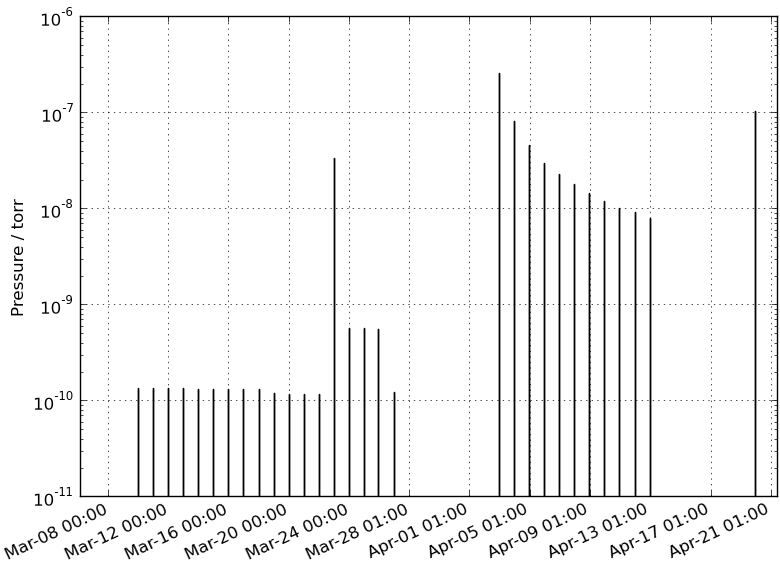
\includegraphics[width=10cm]{morning_pressure.png}
 \caption{ The morning pressure in a vacuum chamber at the department. The
   pressure gauge is unable to read high pressures, and thus no data is
   available from periods where the chamber is vented for maintenance.
   \label{fig:morning_pressure}
 } 
 \end{center}
\end{figure}
Plots like these can be a useful tool to monitor the general health of
the chamber, i.e. if leaks has developed, a valve is failing, a
roughing pump is malfunctioning etc. It should be mentioned that this
is a function that have been sought after for quite some time, but
have simply not been possible before the automated logging and
selective plotting, as it would have required a person to log the data
in the middle of the night and to manually periodically make new plots
of the latest time period.

\subsection{Status of experiments with long durations}

Within our field it is not unusual to have experiments or a
preparation procedures before an experiment running for extended
periods of time i.e. over night, or over several days. Obviously for
such procedures running when no-one is present to monitor it, the
programs that execute the procedure are themselves responsible for the
safety of the system/equipment and for shutting it down if something
unintentional happens. But with the continuous logging, it is now a
simple task to add surveillance to these procedures that alerts the
user if the procedure has been stopped. When this happens, it is then
possible for the operator to access if it is safe to start the
experiment again, even from home. This can help to prevent a loss of
experimentation time if the experiment stopped e.g.\ at the beginning
of a large unsupervised experimentation time like a weekend.

One example where the this is used is for the cleaning of the metal
single crystal samples before experimentation. The cleaning of the
surface is achieved by running a number (5-20) of cleaning
cycles. Each of these cycles can take up to several hours. Before this
task was automatized, it typically required simple manual intervention
2-4 times during a 30 to 120 minute cycle. Obviously, this was a
suboptimal solution, since a lot of time was spent, with only small
time intervals to work on other things, before the next manual
intervention. After the total automation of the task and the
implementation of the surveillance features mentioned above this
procedure can now run e.g.\ for 10-16 hours over night and produce a
sample ready for experimentation at the beginning of the work day.

Another example where we use the monitoring of extended procedures are
in the experiments on the micro-reactors\fixme{insert reference}
setups. For these devices, it is very common to have quite long
experimentation times. They can be used to allow for sufficient system
settle time when parameters have been changed, to study long time
stability effects on the samples or to thoroughly search the parameter
space for the experiment. Obviously, for all these purposes the more
experimentation time the better and being able to un-problematically
and safely utilize nights and weekends is a noticeable
improvement.\fixme{possibly expand}

\subsection{Cooling water alarms}\label{sec:cooling_water_alarms}

Several important pieces of equipment in our lab require cooling. If
the cooling disappears it can result in the break down if this
equipment, which can be quite expensive both in repair cots and lost
equipment up-time.% In our lab the main components with critical cooling
%requirements are the turbo molecular pumps that are used to maintain
%vacuum.

\fixme{Cannot quite evaluate if this transition is to clumsy}
As previously mentioned the access to a centralized point of storage
for experimental data allows for real-time continuous logging of
various parameters used as indicators for system health. Critical
system parameters can hence be monitored and used to trigger alarms
when these fall out of specified ranges. % Furthermore, the logging of
%experimental setup parameters continuously enables access to these
%values at any previous point in time.
To use this feature to implement surveillance of the cooling, we
mounted temperature measurements on all the equipment with critical
cooling requirements and log all of these temperatures via the data
system. This approach has the very desirable side effect that we can
now also monitor the health (to the extent it is given by the
temperature) of each piece of equipment individually to evaluate of
the equipment is getting old or requires maintenance. To implement the
alarms, a program was written that retrieves the latest temperatures
from the database, compares them with values from a certain time
interval back and sends out an alarm via email if they start to
climb. Appropriately coupled with email alarms, e.g.\ on smart-phones,
this feature provides the desired real time notification of critical
cooling loss.
